\clearpage
\chapter{Results}

\section{Result exhaustive search}
    
    \subsection{Training}
    
        
        
    \subsection{Performance}
        
        
    \clearpage
    \begin{figure}[H]
        \centering
        \includegraphics[scale=0.3]{figures/epoch_50_test_38kHz_18kHz_70kHz_120kHz_200kHz_333kHz.png}
        \caption{Overview of the greedy frequency test from all to one single frequency. The red line is the best F1 score during the tests at each stage. Colored blocks indicate the frequencies that resulted in the previously mentioned score.}
      	\medskip 
        \label{test}
    \end{figure}
    %
        \clearpage
    \begin{figure}[H]
        \centering
        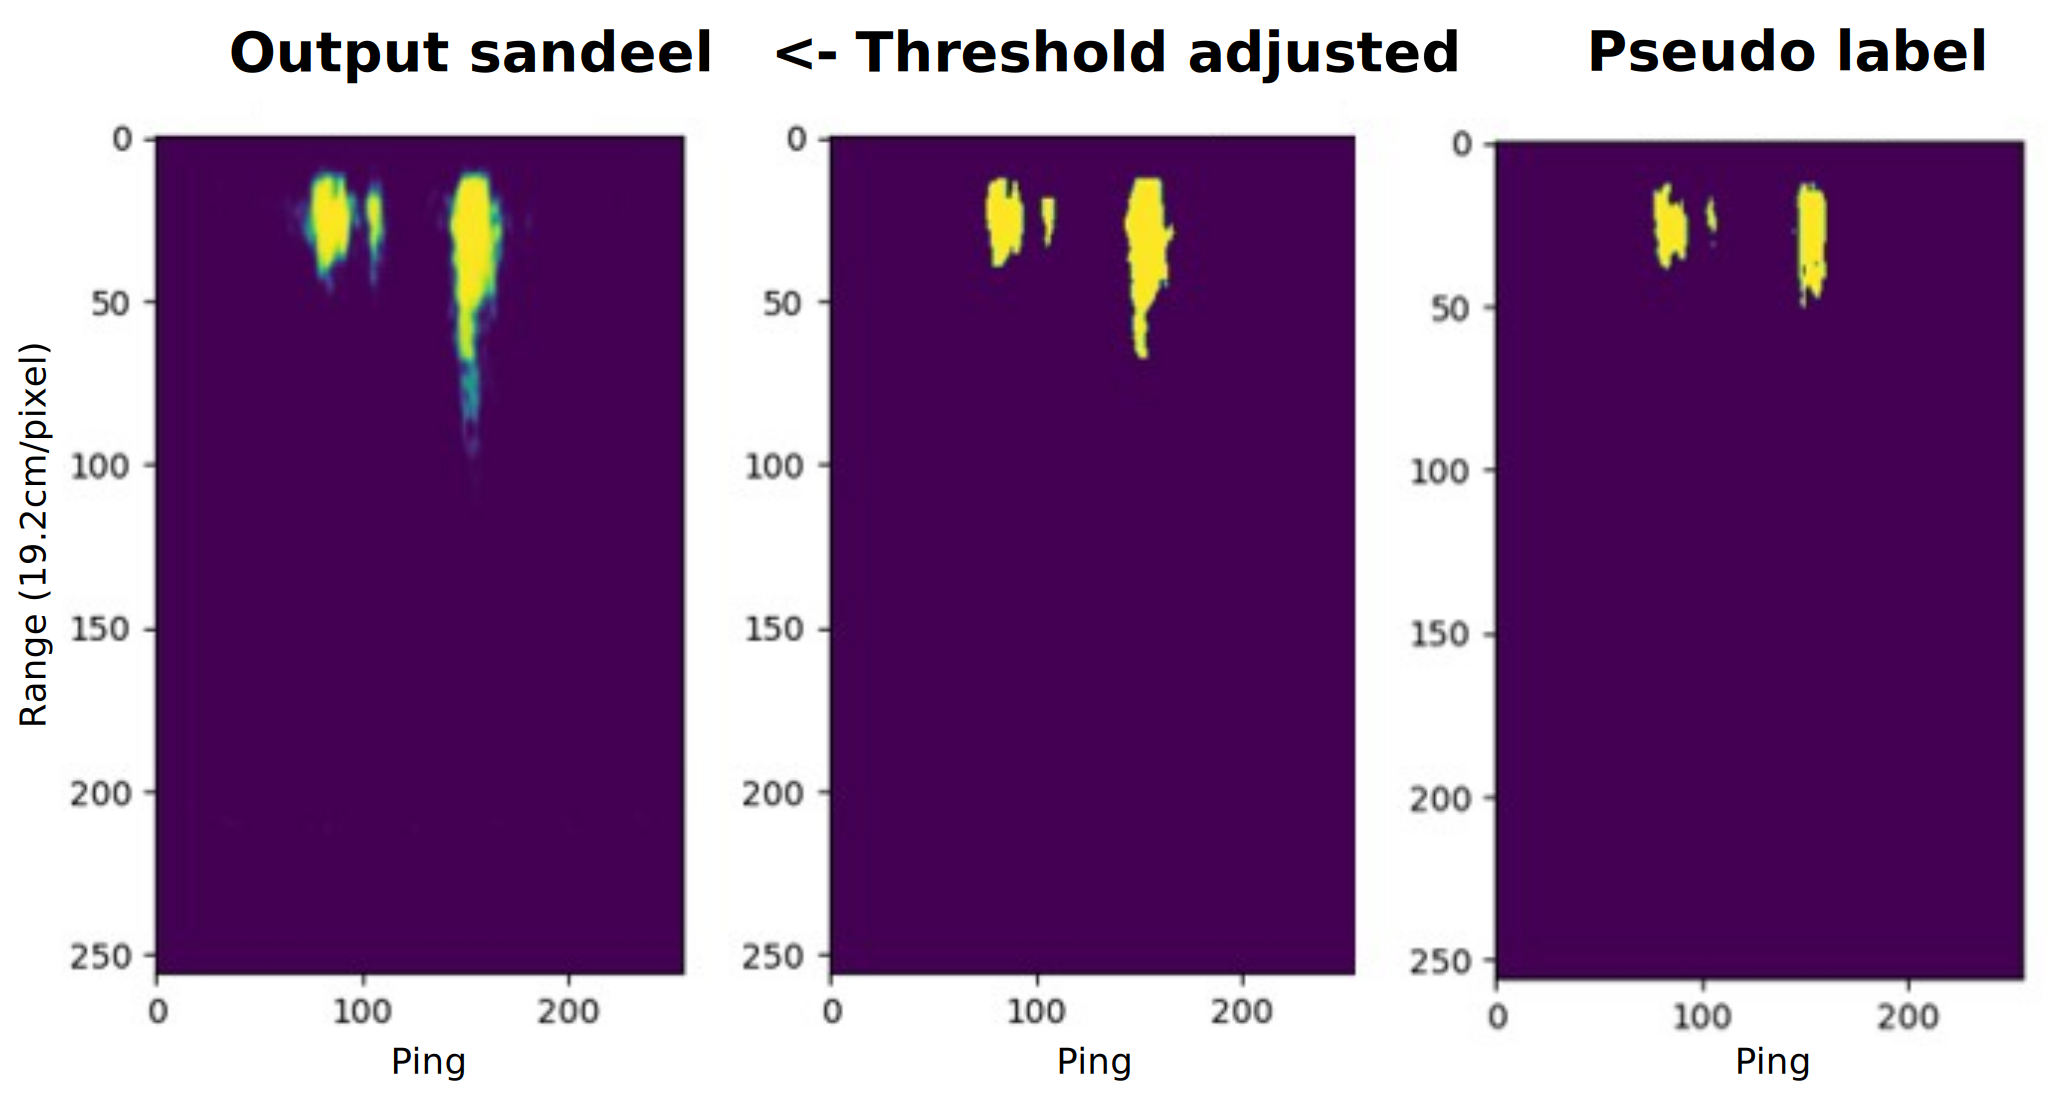
\includegraphics[scale=0.7]{figures/SANDEEL_WITH_LABEL.png}
        \caption{Overview of the greedy frequency test from all to one single frequency. The red line is the best F1 score during the tests at each stage. Colored blocks indicate the frequencies that resulted in the previously mentioned score.}
      	\medskip 
        \label{sandeel_threshold_label}
    \end{figure}
    
    
    
    \clearpage
    \begin{figure}[H]
        \centering
        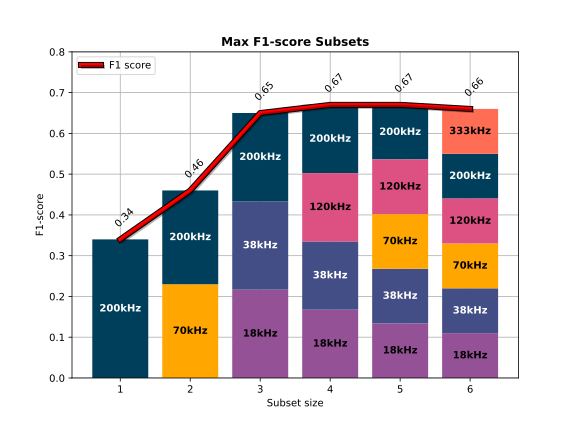
\includegraphics[scale=0.7]{figures/increasing_freq_f1.png}
        \caption{Overview of the greedy frequency test from all to one single frequency. The red line is the best F1 score during the tests at each stage. Colored blocks indicate the frequencies that resulted in the previously mentioned score.}
      	\medskip 
        \label{increasing_freq_f1_score_fig}
    \end{figure}
    
    \begin{figure}[H]
        \centering
        \subfloat[\centering Loss during training]{{\includegraphics[width=5cm]{figures/Loss_val_train.png} }}%
        \qquad
        \subfloat[\centering Recall]{{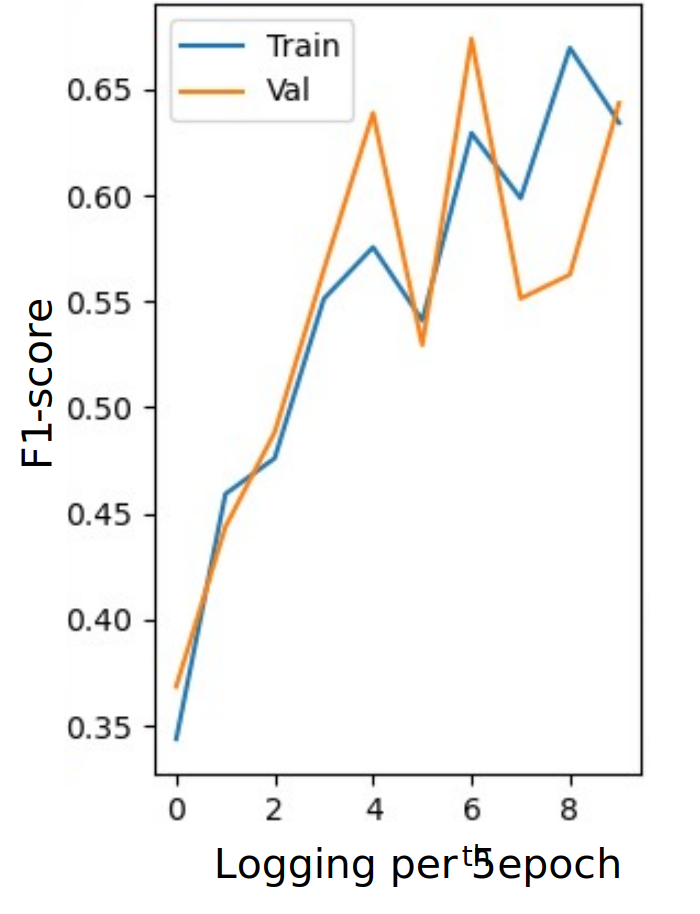
\includegraphics[width=5cm]{figures/F1_score_per_5.png} }}%
        \caption[Loss and F1 score during training]{The F1-score and loss for both training(blue) and validation(orange). The validation loss were calculated less often, resulting in larger steps.}%
        \label{fig:example}%
    \end{figure}
    
    
    % Precision
    \clearpage
    \begin{figure}[H]
        \centering
        \includegraphics[scale=0.7]{figures/increasing_freq_precision.png}
        \caption{Overview of the greedy frequency test from all to one single frequency. The red line is the best F1 score during the tests at each stage. Colored blocks indicate the frequencies that resulted in the previously mentioned score.}
      	\medskip 
        \label{increasing_freq_precision_score_fig}
    \end{figure}

    % Recall
    \clearpage
    \begin{figure}[H]
        \centering
        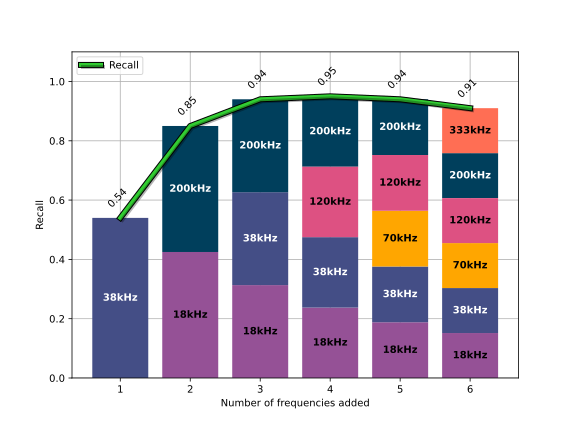
\includegraphics[scale=0.7]{figures/increasing_freq_recall.png}
        \caption{Overview of the greedy frequency test from all to one single frequency. The red line is the best F1 score during the tests at each stage. Colored blocks indicate the frequencies that resulted in the previously mentioned score.}
      	\medskip 
        \label{increasing_freq_recall_score_fig}
    \end{figure}
    
    
        \begin{figure}[H]
        \centering
        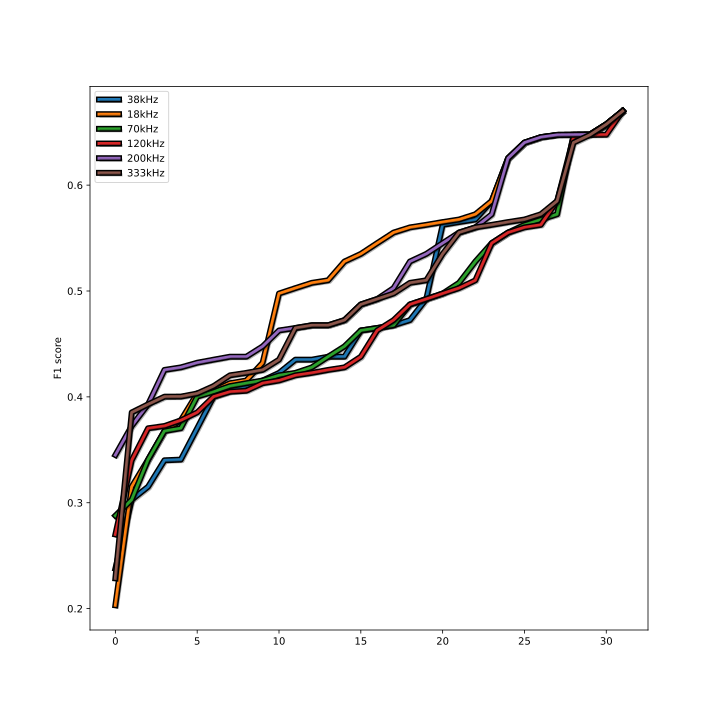
\includegraphics[scale=0.7]{figures/perfomance_trend.png}
        \caption{Overview of the greedy frequency test from all to one single frequency. The red line is the best F1 score during the tests at each stage. Colored blocks indicate the frequencies that resulted in the previously mentioned score.}
      	\medskip 
        \label{performance_trend}
    \end{figure}


